%%%%%%%%%%%%%%%%%%%%%%%%%%%%%%%%%%%%%%%%%%%%%%%%%%%%%%%%%%%%%%%%%%%%%%%%
% Plantilla TFG/TFM
% Escuela Politécnica Superior de la Universidad de Alicante
% Realizado por: Jose Manuel Requena Plens
% Contacto: info@jmrplens.com / Telegram:@jmrplens
%%%%%%%%%%%%%%%%%%%%%%%%%%%%%%%%%%%%%%%%%%%%%%%%%%%%%%%%%%%%%%%%%%%%%%%%

\chapter{Teoría de Antenas}
\par En este capitulo se realizará una breve contextualización sobre el concepto de antena así como un repaso a los parámetros que las caracterizan. Estos conceptos son, por lo general, aplicables a cualquier tipo de antena, en capítulos posteriores se especificará lo aprendido para el caso de las antenas en tecnología microstrip.

\section{Conceptos básicos}

\par Las antenas son transductores entre un medio guaiado y uno radiado. En su diseño más simplificado se analizaría un conductor metálico por el cual fluye una corriente variable en el tiempo. Se entiende como medio guiado a cualquier tipo de línea de transmisión: Cable coaxial, fibra óptica así como guías de onda. Y como medio radiado el aire o el espacio. Las antenas transmisoras serán las encargadas de transformar esta las corrientes eléctricas a \gls{oem}, mientras que las receptoras tomarán las \gls{oem} desde el medio radiado y las convertirán de nuevo a impulsos eléctricos para su posterior procesado. Las primeras antenas fueron diseñadas en 1888 por \textit{Heinrich Hertz} pero no fue hasta 1895 cuando \textit{Guglielmo Marconi} empezó a desarrollar antenas con el objetivo de transmitir información a largas distancias.
\\
\par Como se explico en el \todo{capitulo1}, cualquier variación de un campo eléctrico generará un campo magnético y viceversa. Cuando ambos campos conviven y existen variaciones de estos campos se dice que existe una radiación electromagnética. Para entender el principio de funcionamiento de una antena se tomará como ejemplo el caso de hilo conductor cerrado. Si se introdujera una corriente eléctrica fluctuante en el tiempo dentro del conductor, por el principio de inducción electromagnética (Tercera ecuación de Maxwell, Ley de Faraday-Lentz) se produciría un campo magnético fluctuante y un campo eléctrico asociado a su alrededor, estaríamos hablando de un campo electromagnético. Pero este campo electromagnético no se propagaría y estaría siempre al rededor del conductor cerrado. Para poder propagar las \gls{oem} se debe conseguir separar la onda electromagnética del conductor.
\\
\par Para entender el efecto de separación se tomará como referencia dos cargas eléctricas de distintas polaridades separadas a una distancia determinada (fig. \ref{fig:campo1}), a esto se le conoce como dipolo eléctrico y producirán un campo eléctrico cuyas líneas de fuerza irán del positivo al negativo. Estás dos cargas intentarán juntarse debido al efecto de atracción. En el momento de mayor separación de las cargas, su velocidad será nula y su aceleración máxima. Conforme se vayan acercando la velocidad irá aumentando y la aceleración disminuyendo hasta que en el punto donde se encuentran la velocidad será máxima y la aceleración nula. Suponiendo un escenario teórico sin pérdidas estás cargas estarían fluctuando e intercambiando sus posiciones indefinidamente. Si se analiza el campo eléctrico producido por las cargas mientras estas están fluctuando se observaría como, en vez de seguir encontrando un campo eléctrico simple de menor intensidad, este se deforma debido a la aceleración presente en las cargas. Esta deformación es también conocida como efecto \textit{kink} (fig. \ref{fig:campo2}).
\\
\par Continuando con el experimento se observa como pasado un lapso de un 1/4 del periodo de la oscilación, momento en el que las dos cargas se cruzan en el mismo punto, el campo eléctrico producido es nulo, cerrándose así las líneas de campo que habían sido producidas cuando las partículas estaban aún separadas (fig. \ref{fig:campo3}). Es entonces cuando se produce la propagación y generación del frente de onda del campo eléctrico, con su respectivo campo magnético asociado. Se debe observar como la longitud de la \gls{oem} propagada es exactamente el doble de la longitud existente entre las dos cargas (fig. \ref{fig:campo4}).\\

\begin{figure}[h]
\centering
	\begin{subfigure}[b]{0.3\textwidth} % Espacio horizontal ocupado por la subfigura
		\centering
		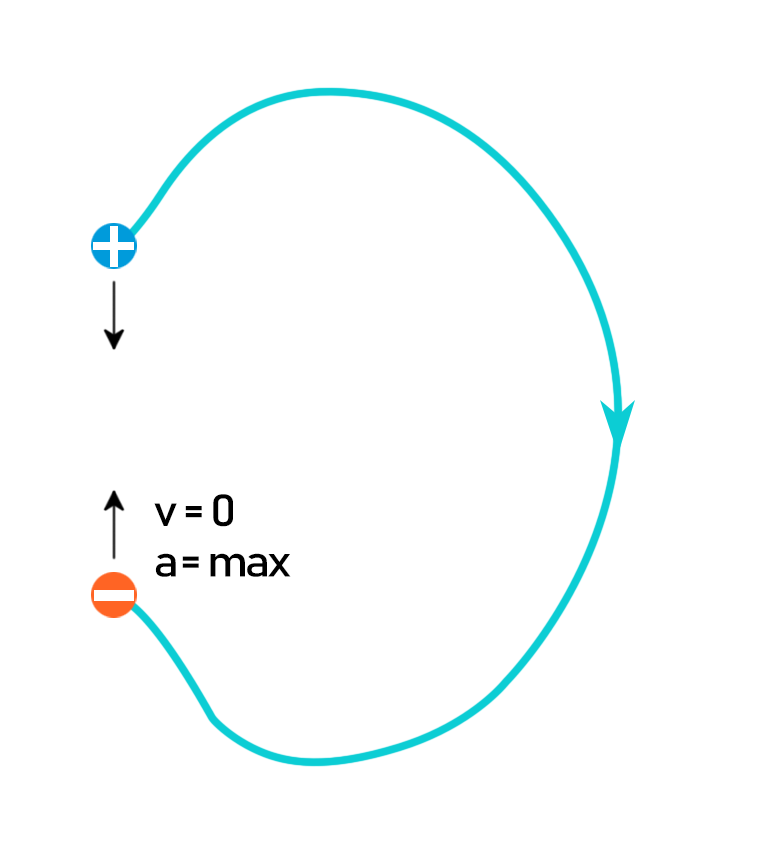
\includegraphics[width=5cm]{archivos/campos/campos1} % Tamaño de la imagen
		\caption{t = 0}
		\label{fig:campo1}
	\end{subfigure}
~ % Añadir el espacio deseado, si se deja la linea en blanco la siguiente subfigura ira en una nueva linea
	\begin{subfigure}[b]{0.3\textwidth} % Espacio horizontal ocupado por la subfigura
	\centering
		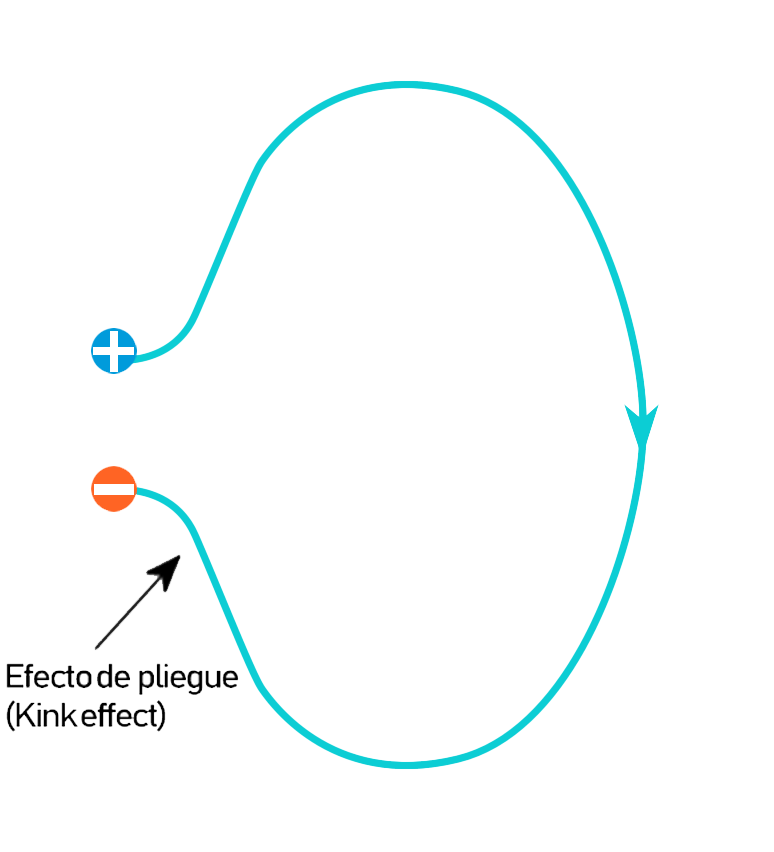
\includegraphics[width=5cm]{archivos/campos/campos2} % Tamaño de la imagen
		\caption{0 < t < T/4}
		\label{fig:campo2}
	\end{subfigure}
	\begin{subfigure}[b]{0.3\textwidth} % Espacio horizontal ocupado por la subfigura
	\centering
		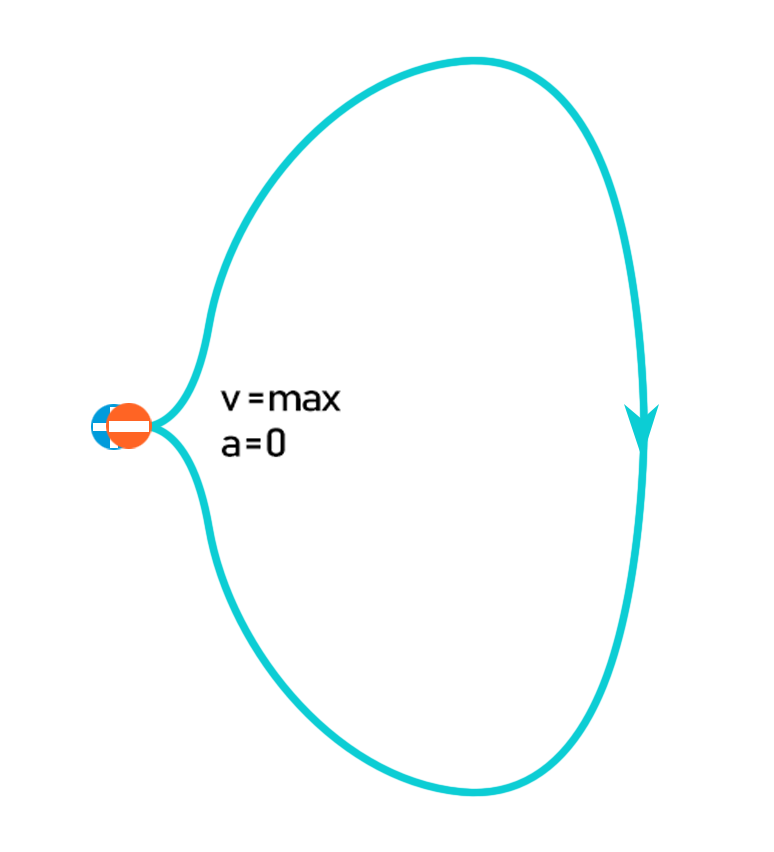
\includegraphics[width=5cm]{archivos/campos/campos3} % Tamaño de la imagen
		\caption{t = T/4}
		\label{fig:campo3}
	\end{subfigure}
	\begin{subfigure}[h]{0.5\textwidth} % Espacio horizontal ocupado por la subfigura
	\centering
	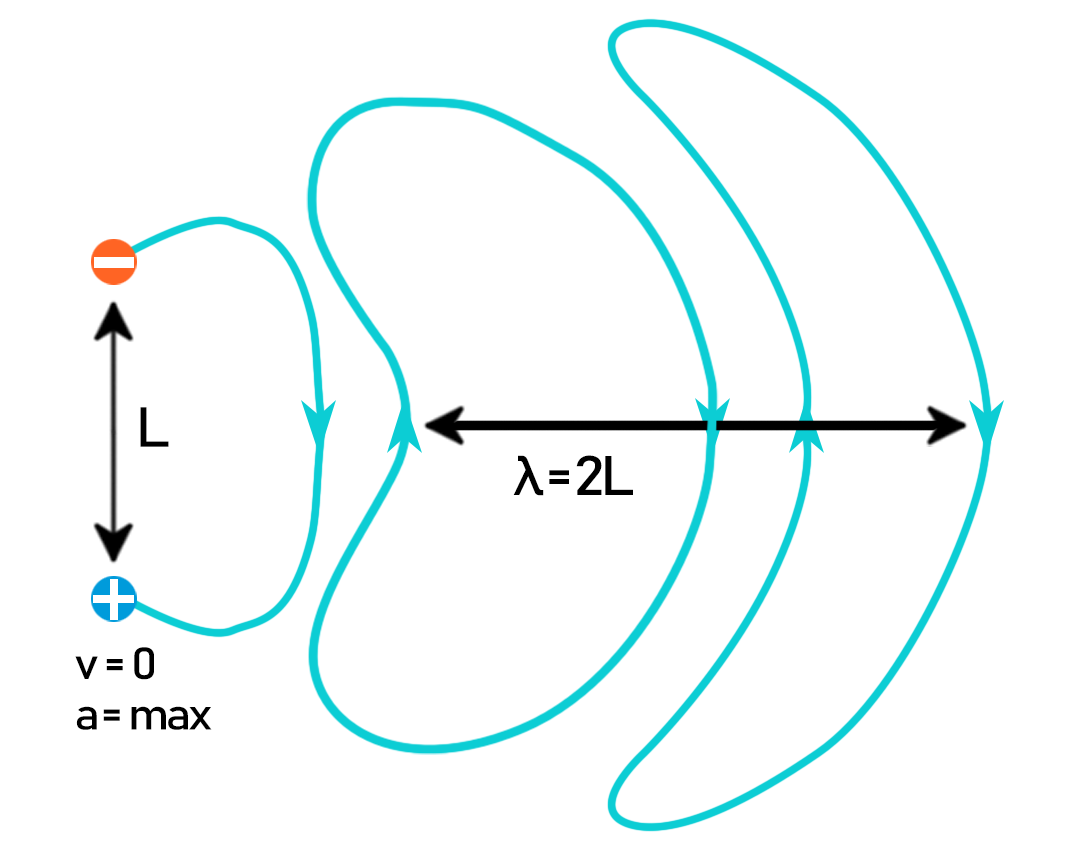
\includegraphics[width=10cm]{archivos/campos/campos4} % Tamaño de la imagen
	\caption{t > T/4}
	\label{fig:campo4}
\end{subfigure}
\caption{Proceso de separación de campo eléctrico}\label{sistemass}
\end{figure}

\par En la práctica se puede simular el experimento en lo que se denomina como antena dipolo, la antena más básica existente, que será estudiada con mayor detenimiento a lo largo de este capítulo. En una antena dipolo, al aplicar una tensión variable sobre los bornes de esta, las cargas irán oscilando de un extremo a otro según la polaridad del generador en ese instante, produciendo campos eléctricos capaces de separarse de la antena, con su consiguiente generación de campos magnéticos. El conjunto de la propagación de ambos campos son los campos electromagnéticos en los que se propagará la \gls{oem}. En la figura \ref{fig:dipolo} se pueden observar ejemplos de antenas dipolo. 

\begin{figure}[h]
\centering
	\begin{subfigure}[b]{0.4\textwidth} % Espacio horizontal ocupado por la subfigura
		\centering
		\includegraphics[width=7cm]{archivos/dipolo/dipole1} % Tamaño de la imagen
		\caption{Esquema de un dipolo}
		\label{fig:dipolo1}
	\end{subfigure}
~ % Añadir el espacio deseado, si se deja la linea en blanco la siguiente subfigura ira en una nueva linea
	\begin{subfigure}[b]{0.4\textwidth} % Espacio horizontal ocupado por la subfigura
	\centering
		\includegraphics[width=7cm]{archivos/dipolo/dipole2} % Tamaño de la imagen
		\caption{Dipolo instalado sobre un poste}
		\label{fig:dipolo2}
	\end{subfigure}
\caption{Antenas dipolo de media onda}\label{fig:dipolo}
\end{figure}

\par El principio básico de diseño de antenas se basa en la geometría de estas. Es importante remarcar que para que la transmisión de la señal aplicada por el generador y que se desea convertir en \gls{oem}, la longitud de los lados del dipolo deben estar relacionados con la longitud de onda de la señal que se desea transmitir. En el caso del dipolo, los extremos tendrán una longitud de $\lambda$/4. Al juntan ambos extremos se puede observar que la antena tendrá una dimensión total de $\lambda$/2, y si se tiene en cuenta que la longitud de onda de la \gls{oem} generada es el doble de la longitud de la antena, se obtendrá una \gls{oem} radiada cuya frecuencia sea idéntica a la aplicada por el generador.
\\
\par Aunque se ha analizado el caso de una antena para que funcione como transmisora, el mismo principio de funcionamiento se aplica cuando queremos que esta funcione como receptora de señales. Una \gls{oem} que viaje por el espacio será capaz de hacer oscilar las cargas de una antena receptora cuando su frecuencia y las longitud de la antena estén directamente relacionadas y se produzca la resonancia sobre esta. La diferencia es que a la salida de la antena receptora no tendremos un generador, sino lo que denominaremos como carga, pudiendo ser esta cualquier tipo de componente eléctrico o electrónico que sea capaz de trabajar con las corrientes eléctricas producidas por la fluctuación de cargas eléctricas en el interior de la antena.

